
%(BEGIN_QUESTION)
% Copyright 2011, Tony R. Kuphaldt, released under the Creative Commons Attribution License (v 1.0)
% This means you may do almost anything with this work of mine, so long as you give me proper credit

Suppose you had a current-to-pressure (``I/P'') transducer with an output range of 3 to 15 PSI and an input range of 4 to 20 mA.  The following calibration table shows several input signal levels and their corresponding percentages of span and output pressures:

% No blank lines allowed between lines of an \halign structure!
% I use comments (%) instead, so that TeX doesn't choke.

$$\vbox{\offinterlineskip
\halign{\strut
\vrule \quad\hfil # \ \hfil & 
\vrule \quad\hfil # \ \hfil & 
\vrule \quad\hfil # \ \hfil \vrule \cr
\noalign{\hrule}
%
% First row
Input signal & Percent of span & Output pressure \cr
%
% Another row
applied (mA) & (\%) & (PSI) \cr
%
\noalign{\hrule}
%
% Another row
6.88 & 18 & 5.16 \cr
%
\noalign{\hrule}
%
% Another row
5.1 & 6.88 & 3.83 \cr
%
\noalign{\hrule}
%
% Another row
12.8 & 55 & 9.6 \cr
%
\noalign{\hrule}
%
% Another row
17.44 & 84 & 13.08 \cr
%
\noalign{\hrule}
%
% Another row
6.53 & 15.83 & 4.9 \cr
%
\noalign{\hrule}
} % End of \halign 
}$$ % End of \vbox

While the calculations for obtaining percent and output pressure (PSI) from input current (mA) values are not very complex, they can be tedious.  A powerful computer-based tool for relieving this tedium is a type of application called a {\it spreadsheet}.  A very common example of spreadsheet software is Microsoft {\it Excel} (although other spreadsheet programs exist, some of them free!).

A spreadsheet program presents a screen full of rectangular {\it cells} into which text, numerical values, and mathematical formulae may be entered.  Each cell is ``addressed'' by a system of row and column designators, traditionally numbers for rows and letters for columns (like the classic game of ``Battleship'' where coordinates on a grid-map are called out by letter and number combination) but a more modern convention designates both rows and columns by number.

We may set up a spreadsheet to calculate percentage values for this I/P based on input currents as follows.  The yellow and blue cell shading (color fill) shown in this example is entirely optional, but helps to distinguish number-entry fields from calculated-value fields (the number in the yellow cell {\tt R2C1} is the milliamp value you type in to the spreadsheet, while the number in the blue cell {\tt R2C3} is the PSI value calculated by the spreadsheet):

$$\includegraphics[width=15.5cm]{i01626x01.eps}$$

What follows is a list of cell entries needed to create the spreadsheet display you see above:

\begin{itemize}
\item{} {\bf Cell R1C1:} {\tt Input (mA)}
\item{} {\bf Cell R2C1:} {\tt 6.88}
\item{} {\bf Cell R1C3:} {\tt Percent}
\item{} {\bf Cell R2C3:} {\tt = (R2C1 - 4) / 16} \hskip 10pt {\it (select ``\%'' display formatting)}
\end{itemize}

The text inside cells R1C1 and R1C3 is not essential for the spreadsheet to function -- like the color shading, they merely serve as labels to help describe what the number values mean.  The formula entered into cell R2C3 begins with an equals sign (=), which tells the spreadsheet to regard it as a formula rather than as text to be displayed verbatim as in R1C1 and R1C3.  Note how the formula references the numerical value located in the ``row 2 column 1'' cell by calling it ``R2C1''.  This allows the user to enter different values into cell R2C1, and the spreadsheet will automatically re-calculate the percentage for each entered mA value.  Thus, if you were to edit the contents of cell R2C1 to hold 12.8 instead of 6.88, the value shown in cell R2C3 would update to display 55.0 instead of 18.0 as it does now.

\vskip 10pt

\vfil \eject

Your first task here is to start up a spreadsheet program and enter what is shown above, then validate the accuracy of your work by entering several different current (milliamp) values and checking that the percentages for each are calculated correctly by the spreadsheet.

Now that you have successfully created this spreadsheet, add the appropriate enteries into cells R1C5 and R2C5 so that it also calculates the appropriate output pressure for the I/P, for any arbitrary input current entered into cell R2C1.  When complete, your modified spreadsheet should look something like this:

$$\includegraphics[width=15.5cm]{i01626x02.eps}$$

Show what entries you had to place into cells R1C5 and R2C5 to make this spreadsheet work. 

\vskip 20pt \vbox{\hrule \hbox{\strut \vrule{} {\bf Suggestions for Socratic discussion} \vrule} \hrule}

\begin{itemize}
\item{} Identify the text character used to represent {\it division} in the formula shown in cell R2C3.  What is the appropriate character to represent {\it multiplication}?
\item{} Explain why parentheses are used in the formula in cell R2C3.  {\it Hint: a good problem-solving approach for answering this question is to analyze what would happen if the parentheses were not there!}
\item{} Explain what would happen if cell R2C3 were not configured to display in {\it percent}.
\item{} There is more than one correct formula to enter into cell R2C5 to properly calculate the output pressure in PSI.  One formula references the percentage value (located at R2C3), while the other formula references the milliamp value (located at R2C1).  Compare these two formulae, and explain which one makes more sense to you.
\item{} Explain how a spreadsheet is such a powerful mathematical tool for performing ``tedious'' calculations such as instrument input/output responses.  Can you think of any other practical uses for a spreadsheet?
\end{itemize}

\underbar{file i01626}
%(END_QUESTION)





%(BEGIN_ANSWER)

Here are two possible formulae for entry into cell R2C5:

\vskip 10pt

{\tt = ((R2C1 - 4) / 16) * 12 + 3}

\vskip 10pt

{\tt = R2C3 * 12 + 3}

\vskip 10pt

One very practical use for this type of spreadsheet program is to create practice problems for yourself, so that you may practice instrument input/output range calculations.

%(END_ANSWER)





%(BEGIN_NOTES)

\vfil \eject

\noindent
{\bf Summary Quiz:}

Calculate the output pressure (3-15 PSI range) from an I/P transducer given a 13 mA input signal (4-20 mA range):

\begin{itemize}
\item{} 13.0 PSI
\vskip 5pt
\item{} 12.75 PSI
\vskip 5pt
\item{} 10.8 PSI
\vskip 5pt
\item{} 9.75 PSI
\vskip 5pt
\item{} 13.4 PSI
\vskip 5pt
\item{} 17.33 PSI
\end{itemize}

%INDEX% Calibration: table, I/P transducer
%INDEX% Computer spreadsheet exercise: introduction to spreadsheet usage
%INDEX% Computer spreadsheet exercise: I/P transducer input/output calculations

%(END_NOTES)


